%\documentstyle[10pt,twoside]{article}
%\documentstyle[twoside]{article}
\documentclass[twoside]{article}
\setlength{\oddsidemargin}{0.25 in}
\setlength{\evensidemargin}{-0.25 in}
\setlength{\topmargin}{-0.6 in}
\setlength{\textwidth}{6.5 in}
\setlength{\textheight}{8.5 in}
\setlength{\headsep}{0.75 in}
\setlength{\parindent}{0 in}
\setlength{\parskip}{0.1 in}

\usepackage{graphicx}
\usepackage{url}

%
% The following commands sets up the lecnum (lecture number)
% counter and make various numbering schemes work relative
% to the lecture number.
%
\newcounter{lecnum}
\renewcommand{\thepage}{\thelecnum-\arabic{page}}
\renewcommand{\thesection}{\thelecnum.\arabic{section}}
\renewcommand{\theequation}{\thelecnum.\arabic{equation}}
\renewcommand{\thefigure}{\thelecnum.\arabic{figure}}
\renewcommand{\thetable}{\thelecnum.\arabic{table}}
\newcommand{\dnl}{\mbox{}\par}

%
% The following macro is used to generate the header.
%
\newcommand{\lecture}[4]{
   \pagestyle{myheadings}
   \thispagestyle{plain}
   \newpage
   \setcounter{lecnum}{#1}
   \setcounter{page}{1}
   \noindent
   \begin{center}
   \framebox{
      \vbox{\vspace{2mm}
    \hbox to 6.28in { {\bf CMPSCI~677~~~Distributed and Operating Systems
                        \hfill Spring 2019} }
       \vspace{4mm}
       \hbox to 6.28in { {\Large \hfill Lecture #1: #2  \hfill} }
       \vspace{2mm}
       \hbox to 6.28in { {\it Lecturer: #3 \hfill Scribe: #4} }
      \vspace{2mm}}
   }
   \end{center}
   \markboth{Lecture #1: #2}{Lecture #1: #2}
   \vspace*{4mm}
}

%
% Convention for citations is authors' initials followed by the year.
% For example, to cite a paper by Leighton and Maggs you would type
% \cite{LM89}, and to cite a paper by Strassen you would type \cite{S69}.
% (To avoid bibliography problems, for now we redefine the \cite command.)
%
\renewcommand{\cite}[1]{[#1]}

% \input{epsf}

%Use this command for a figure; it puts a figure in wherever you want it.
%usage: \fig{NUMBER}{FIGURE-SIZE}{CAPTION}{FILENAME}
\newcommand{\fig}[4]{
            %\vspace{0.2 in}
            \centerline{\includegraphics[scale=#2]{#4}}
            \begin{center}
            Figure \thelecnum.#1:~#3
            \end{center}
    }

% Use these for theorems, lemmas, proofs, etc.
\newtheorem{theorem}{Theorem}[lecnum]
\newtheorem{lemma}[theorem]{Lemma}
\newtheorem{proposition}[theorem]{Proposition}
\newtheorem{claim}[theorem]{Claim}
\newtheorem{corollary}[theorem]{Corollary}
\newtheorem{definition}[theorem]{Definition}
\newenvironment{proof}{{\bf Proof:}}{\hfill\rule{2mm}{2mm}}

% Some useful equation alignment commands, borrowed from TeX
\makeatletter
\def\eqalign#1{\,\vcenter{\openup\jot\m@th
  \ialign{\strut\hfil$\displaystyle{##}$&$\displaystyle{{}##}$\hfil
      \crcr#1\crcr}}\,}
\def\eqalignno#1{\displ@y \tabskip\@centering
  \halign to\displaywidth{\hfil$\displaystyle{##}$\tabskip\z@skip
    &$\displaystyle{{}##}$\hfil\tabskip\@centering
    &\llap{$##$}\tabskip\z@skip\crcr
    #1\crcr}}
\def\leqalignno#1{\displ@y \tabskip\@centering
  \halign to\displaywidth{\hfil$\displaystyle{##}$\tabskip\z@skip
    &$\displaystyle{{}##}$\hfil\tabskip\@centering
    &\kern-\displaywidth\rlap{$##$}\tabskip\displaywidth\crcr
    #1\crcr}}
\makeatother

% **** IF YOU WANT TO DEFINE ADDITIONAL MACROS FOR YOURSELF, PUT THEM HERE:

\newcommand{\que}[1]{\textbf{Question:} #1\\}
\newcommand{\ans}[1]{\textbf{Answer:} #1\\}

% Some general latex examples and examples making use of the
% macros follow.

\begin{document}

%FILL IN THE RIGHT INFO.
%\lecture{**LECTURE-NUMBER**}{**DATE**}{**LECTURER**}{**SCRIBE**}
\lecture{5}{February 6}{Prashant Shenoy}{\textbf{Deokgi Hong (2019), Ao Liu (2018)}}

\section{Case studies (Lecture 4: Module 3)}

\subsection{Condor}
Condor uses idle cycles on workstations in a LAN environment. It can be used to run large batch jobs and long simulations. Whenever a user does not use their machines, machines will contact the condor server for work. When the user comes back, the job is suspended like Sprite. Condor supports process migration.

\subsection{Replicated Web Server}
A large website which runs on multiple machines typically has a dispatcher node (or a master node). HTTP requests are queued and the master node assigns those requests to one of other machines. The master node runs a distributed request scheduler for each HTTP request. Different policies are used for the load balancing such as least loaded, round robin, or session-based policies.

\section{Virtualization}
Virtualization uses or extends an existing interface to mimic the behaviour of another system. It is introduced in 1970s by IBM to run old software on newer mainframe hardware. It provided a software layer which emulates an old hardware, so an old software could be run on top of the software layer.

\que{Do mainframe machines have an operating system?}
\ans{Yes, OS/360 and many generations of it. Early versions of UNIX came out from those OSes.}
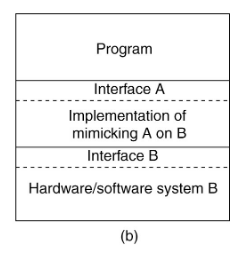
\includegraphics[scale=0.5]{virtlayer.png}

\que{What part of the image is the software layer?}
\ans{The part between Interface A and B. That is the virtualization layer and it is implemented in software.}

\subsection{Type of Interfaces}
\begin{itemize}
\item Assembly instructions (Hardware virtualization)
\item System calls (OS-level virtualization)
\item APIs (Application-level virtualization)
\end{itemize}

\subsection{Type of Virtualization}

\subsubsection{Emulation}

In emulation, a virtual machine (VM) fully emulates every aspects (CPU, a disk, a network interface card) of other machine. It is fully implemented in software.

Examples: Bochs, VirtualPC for Mac, QEMU.

\subsubsection{Full/Native Virtualization}

The VM does not emulate the entire machine, but it emulates enough hardware to run another system. This is typically done when an emulated interface and a native interface are the same. For example, two interfaces might have the same CPU interface. VirtualBox is a software implementation of an Intel machine. It emulates Intel on Intel and allows you to run a whole different OS inside that emulated machine.

Examples: IBM VM family, VMWare Workstation, Parallels, VirtualBox.

\subsubsection{Para-virtualization}

The VM does not simulate hardware. Previous two virtuliazation techniques can use unmodified guest OSes. But in here, the guest OS is modified to support virtualization.

Examples: Xen, VMWare ESX Server.

\subsubsection{OS-level Virtualization}

One OS interface can emulate another OS interface. If you develop an application for Linux 4.2, and there are small changes in the OS interface of Linux 4.3, this might cause breaks of the application. If an OS supports OS-level virtualization, it can emulate older versions of OS. VMs usually mean hardware virtualization and containers usually mean OS-level virtualization.

Examples: Solaris Containers, BSD Jails, Linux Vserver, Linux containers, Docker.

\subsubsection{Application level virtualization}

One application library can be used to emulate the other. One example is JVM. JVM is an abstract machine which might be written in C++ or C libraries, and all Java codes run on JVM. Rosetta on Mac is another example. It takes a PowerPC executable and does dynamic translation to x86 instructions.

Example: JVM, Rosetta on Mac (also emulation), WINE.

\que{Does it (translation) impact on processor speed?}
\ans{Yes. All forms of virtualization are going to impact performance because virtualization needs translation and translation cause overhead.}

\que{In Rosetta, why can't the translation happen before its run?}
\ans{There are many ways to do translations. They chose to do it on runtime because you don't need to do anything to the application. Also, doing static translation is much harder than runtime translation.}

\section{Type of Hypervisors}

Hardware virtualization layer is called a hypervisor or a virtual machine monitor (VMM). There are two types of hypervisors: Type 1 and Type 2.

Type 1: There is no OS to boot, but Type 1 hypervisor. It takes roles of a kernel in the virtualization context. It provides an abstraction of VMs. Multiple OSes can be run on Type 1 hypervisor. An OS does not know the presence of the hypervisor or other VMs. The OS thinks that it is running on real hardware. Type 1 hypervisor is often used in servers or clouds. VMware ESXi is one example.

\que{Can you do further virtualization?}
\ans{Yes, but it is complicated. It is called nested virtualization which is not covered in this course.}

Type 2: It boots to a normal OS. Type 2 hypervisor provides an emulation of hardware. Different OSes on multiple VMs can be run. The OS which runs inside a VM is called a guest OS. Examples of Type 2 hypervisor are VirtualBox, VMWare Workstation and Parallels.

\que{In Type 1, do OSes run in parallel concurrently or do they switch between them?}
\ans{Hypervisor behaves like an OS. It schedules VMs not processes. If you have only one core, it will give time slices to VMs. Other scheduling will be done inside the OS.}

\que{In Type 2, is a guest OS being scheduled as a process?}
\ans{Host OS will treat each VM as a single application process and run a normal CPU scheduling.}

\que{How is it (Type 2 hypervisor) running on the host OS?}
\ans{It is emulating the x86 interface using another x86 interface. But it doesn't run natively on that x86 interface. It will be covered in two slides.}

\que{If you add another guest OS, would you need another Type 2 hypervisor?}
\ans{Think of this hypervisor as a layer. You can run multiple VMs on top of it. But from an OS's perspective, it looks like an independent process. Guest OS 1 looks like process 1, and guest OS 2 looks like process 2. So the same core of that hypervisor is present in both processes. In that sense, you can think of them as distinct, but they are actually the same layer.}

\subsection{How Virtualization Works?}
CPU can run in either user mode (ring 3) or kernel mode (ring 0). In kernel mode, any instructions can be run. But in user mode, only a subset of instructions is allowed to run. OS kernel is trusted than user applications, so OS kernel is run in kernel mode and user applications are run in user mode to limit instruction sets. Simple example is the halt instruction which is not allowed to user applications to run. Also, memory management instruction is only allowed to run in kernel mode. 

Intel CPU has intermediate rings (ring 1, ring 2) in which guest OSes can be run.

Sensitive instructions (I/O, MMU, halt, etc.) are only allowed to run in kernel mode.

Privileged instructions cause a trap or interrupt. I/O is one example. These are not related to user mode or kernel mode.

Type 1 virtualization is only possible on processors where the sensitive instructions are a subset of the privileged instruction. Type 1 hypervisor is the most trusted and controls all the resources so it is run in kernel mode (ring 0). User processes inside any OS are the least trusted, so they are run in user mode (ring 3). OSes are run in user mode. If sensitive instructions are a subset of privileged instructions, sensitive instructions such as I/O cause a trap which is handled in the hypervisor in kernel mode. If CPU does not support it and ignore sensitive instructions, Type 1 hypervisor is not possible. Recent CPUs support this hardware support (Intel VT, AMD SVM). If you turn on this feature, it will create a bitmap for instructions which cause trap. If a bit is set and the instruction is executed in user mode, it will create a trap.

\que{(Inaudible) In general, are sensitive instructions the same as privileged instructions?}
\ans{These are two different concepts. Privileged instructions are simply the ones that cause traps. Sensitive instructions are the ones that are allowed to run in kernel mode.}

\subsection{Type 1 Hypervisor}

In this type, unmodified OS is running in user mode (or ring 1), but it thinks it's running in kernel mode (\textit{virtual kernel mode}). The guest OS traps on privileged instructions and uses VT to trap sensitive instructions. Under this mode, hypervisor is the "real kernel". Upon trap, it executes privileged operations or emulates what the hardware would do.

\que{If the guest OS wants to manage its memory, will it cause a trap?}
\ans{Yes, a trap is handled by the hypervisor.}

\que{Can a guest OS manage other VM's memory?}
\ans{No.}

\que{Does a hypervisor decide what a VM can control?}
\ans{Actually, memory management is implemented in hardware in most cases because of performance. Basically, when you try to access some memory addresses that do not belong to your legal address space, you are not allowed to do it by hardware. It is the same way that one process cannot access another process's memory.}

\que{Does the guest OS see all the resources that it would normally see?}
\ans{Type 1 hypervisor allocate some resources to that VM. If the host has 4 cores and the hypervisor allocates one core to the VM, the OS only sees one core.}

\que{When does it try to access another processor's memory?}
\ans{It will not be allowed to do it because it is limited in what it can see. The same thing happens in a process.}

\que{Is the bit vector configured in the hypervisor?}
\ans{No. That bit vector has to be configured on the processor. This hardware feature can be turn on in BIOS when you boot up.}

\subsection{Type 2 Hypervisor}

Type 2 hypervisor runs as a normal process on the host OS. Guest OS runs as a normal process as well, and it is the same process as the hypervisor because a part of the hypervisor is part of that guest OS. Guest OS runs in user mode and host OS runs in kernel mode. Type 2 hypervisor does binary translation. It scans codes and whenever the hypervisor sees sensitive instructions, they are replaced with function calls on-the-fly. Those functions emulate whatever that instructions wanted to do by making system calls to the actual OS. Traps are not used in this case, so Type 2 hypervisor does not require hardware supports.

\que{Is this the reason you are going to see a slowdown?}
\ans{This is virtualization overhead which incurs significant performance penalty.}

\que{Can Type 2 hypervisor use Intel VT?}
\ans{Optimization of Intel VT normally wouldn't help. But some of Intel VT's additional features might improve performance.}

\que{If the host OS has a certain amount of RAM, what does the guest OS see what part of the RAM?}
\ans{The guest OS gets as much RAM as it has been allocated by the user.}

\que{How does the Type 2 hypervisor allocate dedicated resources?}
\ans{Typically, Type 2 hypervisor is a process. It does not really get dedicated resources.}

\que{If you allocate a certain amount of max memory, can other processes encroach on it?}
\ans{The max is not the same as min. Max doesn't mean you will get that all the time. That means you cannot get more than that. It doesn't mean dedicated amount.}

\que{Does Type 2 hypervisor run as a user process in virtual memory?}
\ans{Yes. You can also swap from disk.}

\subsection{Para-virtualization}

It was developed as a workaround for Type 1 hypervisor that is needed to run on old hardware which does not cause traps on sensitive instructions.

Both type 1 and 2 hypervisors work on unmodified OS. In contrast, para-virtualization modifies OS kernel to replace all sensitive instructions with hypercalls. Thus, OS behaves like a user program making system calls and hypervisor executes the privileged operation invoked by hypercall.

\section{Memory virtualization}

If your guest OS tries to change the memory allocation of a process, that is a sensitive instruction because only the OS is allowed to change page tables. Processes are not allowed to this. But a guest OS in Type 1 does not have those privileges. It still maintains page tables, and it still thinks it owns the machine that it can do whatever it wants, but it is not allowed to do so. So what we do here is that we change those page tables in guest OSes to be read-only. When OS tries to write to that page table, a trap is created because that is a write instruction to read-only memory page. The hypervisor maintains a second page table which is called a shadow page table. That is a mirror of the original page table. It makes those changes in its actual page table. It utilizes the existing hardware feature that causes a trap when a write instruction happens on read-only region.

\que{Is this only for Type 1 hypervisor?}
\ans{Yes. Type 2 hypervisor does binary translation to achieve the same thing.}

\end{document}
